% ============================================================
%  MARL Jammer Drone System — Mid-Semester Evaluation
%  Multi-Agent Reinforcement Learning for Cooperative Swarm Disruption
% ============================================================
\documentclass[10pt, aspectratio=169]{beamer}
\usetheme[progressbar=frametitle]{metropolis}
\usepackage{appendixnumberbeamer}
\usepackage{booktabs}
\usepackage{pgfplots}
\usepgfplotslibrary{dateplot}
\usepackage{graphicx}
\usepackage{tikz}
\usetikzlibrary{positioning, arrows.meta, calc, shapes.geometric, fit, backgrounds}
\usepackage{multirow}
\usepackage{amsmath}
\usepackage{amssymb}
\usepackage{caption}
\usepackage{array}
\usepackage{colortbl}
\pgfplotsset{compat=1.18}
\captionsetup[figure]{labelfont={footnotesize, bf}}

% ── Custom Theme Colors ──
\definecolor{MARLBlue}{HTML}{1B3A5C}
\definecolor{DeepNavy}{HTML}{0D1B2A}
\definecolor{CyberTeal}{HTML}{00838F}
\definecolor{SignalOrange}{HTML}{FF6B35}
\definecolor{JammerGreen}{HTML}{52B788}
\definecolor{White}{HTML}{FFFFFF}
\definecolor{LightGray}{HTML}{F5F5F5}
\definecolor{AlertRed}{HTML}{D62828}
\definecolor{GoldHighlight}{HTML}{E6A817}

\setbeamercolor{frametitle}{bg=DeepNavy}
\setbeamercolor{progress bar}{bg=JammerGreen, fg=DeepNavy}
\setbeamercolor{alerted text}{fg=SignalOrange}
\setbeamercolor{block title}{bg=MARLBlue, fg=White}
\setbeamercolor{block title example}{bg=CyberTeal, fg=White}
\setbeamercolor{block title alerted}{bg=AlertRed, fg=White}
\setbeamercolor{block body}{bg=LightGray}
\setbeamerfont{institute}{size=\large}
\metroset{titleformat=smallcaps, progressbar=foot}

% ── Title Page Info ──
\title{Countermeasures and Defence Mechanisms\\for Drone Swarm Threats}
\subtitle{Major Project (CS499) --- Mid-Semester Evaluation}
\date{13 March 2026}
\author{
  \textbf{Group III}\\[4pt]
  Mrutyunjay Kumar Rao (22CSE1019)\\
  Nischay Khobragade (22CSE1023)\\[6pt]
  {\small \textbf{Guide:} Dr.\ Pravati Swain}
}
\institute{
\begin{minipage}{0.115\textwidth}
\includegraphics[width=\linewidth]{NIT_LOGO_512.png} 
\end{minipage}% <-- The % symbol prevents unwanted extra spaces
\hspace{0.03\textwidth}% Controls the gap between the logo and text
\begin{minipage}{0.84\textwidth}
\raggedright % Forces left-alignment instead of centering
\Large \textbf{National Institute of Technology Goa}\\[2pt]
\small Department of Computer Science and Engineering
\end{minipage}
}

% ── CUSTOM TITLE PAGE LAYOUT OVERRIDE ──
\setbeamertemplate{title page}{
    \vspace*{-0.5cm}
    
    % 1. Logo & Institute at the top
    {\usebeamerfont{institute}\insertinstitute\par}
    
    \vspace{0.1cm} 
    
    % 2. Title & Subtitle
    % Changed \LARGE to \Large to make it slightly smaller
    {\usebeamercolor[fg]{title}\LARGE \textbf{\inserttitle}\par}
    \vspace{0.1cm}
    {\usebeamercolor[fg]{subtitle}\large \insertsubtitle\par}
    
    \vspace{0cm}
    % Separator Line
    \noindent\textcolor{DeepNavy}{\rule{\textwidth}{1.5pt}}\par
    \vspace{0cm}
    
    % 3. Author Info & Date (Side-by-side using minipage)
    \begin{minipage}[t]{0.65\textwidth}
        {\usebeamercolor[fg]{author}\normalsize\insertauthor}
    \end{minipage}%
    \begin{minipage}[t]{0.35\textwidth}
        \raggedleft % Aligns the date to the right side
        {\usebeamercolor[fg]{date}\normalsize\insertdate}
    \end{minipage}\par
}
\begin{document}

% ============================================================
% TITLE PAGE
% ============================================================
% Using [plain] removes the progress bar from overlapping your custom title page
\begin{frame}[plain]
    \maketitle
\end{frame}

% ============================================================
% OVERVIEW & STRUCTURE
% ============================================================
\begin{frame}{Overview \& Structure}
\begin{enumerate}\setlength\itemsep{0.7em}

  \item \hyperlink{sec:recap}{\textbf{Phase 1 Recap \& Limitations}}\\
        \small Where Phase 1 ended and why it was not enough.

  \item \hyperlink{sec:graph}{\textbf{Communication Graph \& Fiedler Value}}\\
        \small Modeling the swarm as a graph; algebraic connectivity $\lambda_2$.

  \item \hyperlink{sec:system}{\textbf{System Pipeline \& DBSCAN Deployment}}\\
        \small Complete 4-phase architecture and intelligent jammer initialization.

  \item \hyperlink{sec:agents}{\textbf{Agent Design — Observation, Actor \& Critic}}\\
        \small 5D state vector, neural network architectures, and CTDE.

  \item \hyperlink{sec:training}{\textbf{Reward Function \& TD Learning}}\\
        \small Multi-objective reward and temporal difference error.

\end{enumerate}
\end{frame}

% ============================================================
\section{I : Phase 1 Recap \& Limitations}\label{sec:recap}
% ============================================================

\begin{frame}{Where Phase 1 Ended --- and Why It Was Not Enough}
\begin{columns}[T,onlytextwidth]
\column{0.48\textwidth}
\begin{block}{What Phase 1 Achieved}
  \small
  \renewcommand{\arraystretch}{1.3}
  \setlength{\tabcolsep}{4pt}
  \begin{tabular}{|l|l|}
  \hline
  \textbf{Component} & \textbf{Phase 1 Approach} \\
  \hline
  Algorithm & Q-Learning + Tile Coding \\ \hline
  Reward    & Max received jamming power \\ \hline
  Scenarios & 2v3, 4v3, 6v3 \\
  \hline
  \end{tabular}
\end{block}

\column{0.48\textwidth}
\begin{alertblock}{Critical Limitations}
  \small
  \begin{itemize}
    \item \alert{Wrong objective} --- maximizing power at individual drones does not measure swarm coordination loss.
    \item \alert{No graph metric} --- no way to know if the swarm is still connected as a network.
    \item \alert{Q-table cannot scale} --- state space explodes beyond 6 agents.
    \item \alert{Single frequency} --- only 2.4\,GHz; real swarms use multiple bands.
  \end{itemize}
\end{alertblock}
\end{columns}

\vspace{0.3cm}
\begin{exampleblock}{Core Gap}
  \centering\small
  High jamming power at individual drones $\neq$ swarm fragmentation\\[4pt]
  \textbf{Phase 2 objective:} prove and optimize the \alert{exact mathematical condition} for swarm disconnection.
\end{exampleblock}
\end{frame}

% ============================================================
\section{II : Communication Graph \& Algebraic Connectivity}\label{sec:graph}
% ============================================================

\begin{frame}{Enemy Swarm $\rightarrow$ Communication Graph $G = (V, E)$}
\begin{columns}[T,onlytextwidth]
\column{0.48\textwidth}
\vspace{0.2cm}
% --- TikZ graph diagram ---
\begin{center}
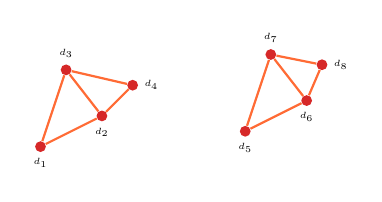
\begin{tikzpicture}[
    drone/.style={circle, fill=AlertRed, minimum size=6pt, inner sep=0pt},
    link/.style={SignalOrange, thick},
    scale=0.65, every node/.style={scale=0.65}
]
  % Cluster 1
  \node[drone] (d1) at (0,0) {};
  \node[drone] (d2) at (1.2,0.6) {};
  \node[drone] (d3) at (0.5,1.5) {};
  \node[drone] (d4) at (1.8,1.2) {};
  % Cluster 2
  \node[drone] (d5) at (4.0,0.3) {};
  \node[drone] (d6) at (5.2,0.9) {};
  \node[drone] (d7) at (4.5,1.8) {};
  \node[drone] (d8) at (5.5,1.6) {};
  % Links within clusters
  \draw[link] (d1)--(d2); \draw[link] (d2)--(d3);
  \draw[link] (d2)--(d4); \draw[link] (d3)--(d4);
  \draw[link] (d1)--(d3);
  \draw[link] (d5)--(d6); \draw[link] (d6)--(d7);
  \draw[link] (d7)--(d8); \draw[link] (d6)--(d8);
  \draw[link] (d5)--(d7);
  % Labels
  \node[below=2pt, font=\tiny] at (d1) {$d_1$};
  \node[below=2pt, font=\tiny] at (d2) {$d_2$};
  \node[above=2pt, font=\tiny] at (d3) {$d_3$};
  \node[right=2pt, font=\tiny] at (d4) {$d_4$};
  \node[below=2pt, font=\tiny] at (d5) {$d_5$};
  \node[below=2pt, font=\tiny] at (d6) {$d_6$};
  \node[above=2pt, font=\tiny] at (d7) {$d_7$};
  \node[right=2pt, font=\tiny] at (d8) {$d_8$};
\end{tikzpicture}
\end{center}

\vspace{0.1cm}
\footnotesize
$V = \{d_1, d_2, \ldots, d_n\}$ --- drones are nodes\\
$E = \{(i,j)\}$ --- active radio links are edges\\[6pt]
\textbf{Adjacency Matrix} (5$\times$5 subset):\\[2pt]
$A = \begin{pmatrix}
0 & 1 & 1 & 0 & 0\\
1 & 0 & 1 & 0 & 0\\
1 & 1 & 0 & 1 & 0\\
0 & 0 & 1 & 0 & 1\\
0 & 0 & 0 & 1 & 0
\end{pmatrix}$

\column{0.50\textwidth}
\begin{block}{\small Edge Condition --- FSPL Model}
  \footnotesize
  \[
    P_R(i,j) = P_{tx} \cdot \left(\frac{c}{4\pi f \cdot d_{ij}}\right)^{2}
  \]
  Edge exists if:
  \begin{itemize}\scriptsize
    \item $P_R(i,j) \geq P_{\text{sens}} = -90\;\text{dBm}$
    \item AND link is \alert{not actively jammed}
  \end{itemize}
  \scriptsize $d_{ij} = \| \mathbf{x}_i - \mathbf{x}_j \|_2$
\end{block}

\vspace{0cm}
\begin{exampleblock}{\small Graph Laplacian}
  \footnotesize
  \[
    L = D - A
  \]
  \vspace{-0.6cm}
  \begin{itemize}\scriptsize
    \item $D$ = diagonal degree matrix
    \item $D[i,i]$ = number of links drone $i$ has
    \item $L$ encodes the \alert{complete connectivity structure} of the swarm
  \end{itemize}
\end{exampleblock}
\end{columns}

\vspace{0cm}
\centering\footnotesize\textit{Recomputed every timestep as jammers move and links break.}
\end{frame}

% ──────────────────────────────────────────────────────────────
\begin{frame}{Algebraic Connectivity $\lambda_2$ --- One Number That Measures Swarm Coordination}
\vspace{0.1cm}
\begin{block}{Eigen decomposition of the Laplacian $L$}
  \centering\small
  $L \cdot \mathbf{v} = \lambda \cdot \mathbf{v}$\qquad
  Eigenvalues: $0 = \lambda_1 \leq \lambda_2 \leq \lambda_3 \leq \cdots \leq \lambda_n$\\[4pt]
  $\lambda_2$ = \textbf{Fiedler Value} = \textbf{Algebraic Connectivity}
\end{block}
\vspace{-0.2cm}
\begin{columns}[T,onlytextwidth]
\column{0.32\textwidth}
\begin{alertblock}{\centering Dense Graph}
  \centering\small
  % Fully connected mini-graph
  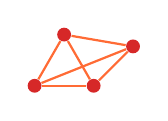
\begin{tikzpicture}[
      drone/.style={circle, fill=AlertRed, minimum size=5pt, inner sep=0pt},
      link/.style={SignalOrange, thick},
      scale=0.5
  ]
    \node[drone](a) at (0,0){};
    \node[drone](b) at (1.5,0){};
    \node[drone](c) at (0.75,1.3){};
    \node[drone](d) at (2.5,1){};
    \draw[link](a)--(b); \draw[link](a)--(c); \draw[link](b)--(c);
    \draw[link](b)--(d); \draw[link](c)--(d); \draw[link](a)--(d);
  \end{tikzpicture}\\[4pt]
  $\lambda_2 = 0.82$\\
  Swarm fully coordinated\\
  \alert{Dangerous}
\end{alertblock}

\column{0.32\textwidth}
\begin{block}{\centering Sparse Graph}
  \centering\small
  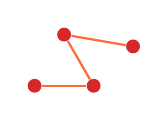
\begin{tikzpicture}[
      drone/.style={circle, fill=AlertRed, minimum size=5pt, inner sep=0pt},
      link/.style={SignalOrange, thick},
      scale=0.5
  ]
    \node[drone](a) at (0,0){};
    \node[drone](b) at (1.5,0){};
    \node[drone](c) at (0.75,1.3){};
    \node[drone](d) at (2.5,1){};
    \draw[link](a)--(b); \draw[link](c)--(d);
    \draw[link](c)--(b);
  \end{tikzpicture}\\[4pt]
  $\lambda_2 = 0.21$\\
  Partially disrupted\\
  \textbf{Degraded}
\end{block}

\column{0.32\textwidth}
\begin{exampleblock}{\centering Fragmented}
  \centering\small
  
\begin{tikzpicture}[
      drone/.style={circle, fill=AlertRed, minimum size=5pt, inner sep=0pt},
      link/.style={SignalOrange, thick},
      scale=0.5
  ]
    \node[drone](a) at (0,0){};
    \node[drone](b) at (1.5,0){};
    \node[drone](c) at (0.75,1.3){};
    \node[drone](d) at (2.5,1){};
  \end{tikzpicture}\\[4pt]
  $\lambda_2 = 0.00$\\
  Swarm fragmented\\
  \textbf{\textcolor{JammerGreen}{Mission Complete}}
\end{exampleblock}
\end{columns}

\vspace{0.3cm}
\begin{center}
\fcolorbox{GoldHighlight}{LightGray}{%
  \parbox{0.88\textwidth}{%
    \centering\small
    \textbf{Proposition 1 --- Fiedler (1973):}\quad
    $\lambda_2(G) = 0 \iff G\text{ is disconnected}$\quad;\quad
    $\lambda_2(G) > 0 \iff G\text{ is connected}$\\[3pt]
    When our system drives $\lambda_2$ to zero, swarm fragmentation is \alert{provably guaranteed}.
  }%
}
\end{center}
\end{frame}

% ============================================================
\section{III : System Pipeline \& DBSCAN Deployment}\label{sec:system}
% ============================================================

\begin{frame}{Complete System Pipeline --- 4 Phases}
\begin{columns}[T,onlytextwidth]
\column{0.62\textwidth}
\vspace{-0.1cm}
\begin{center}
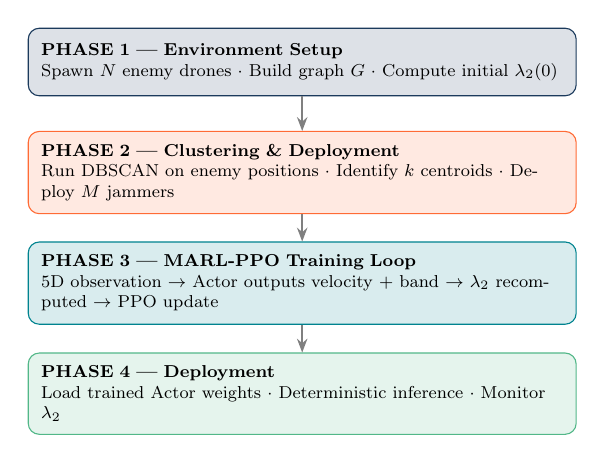
\begin{tikzpicture}[
    box/.style={rectangle, rounded corners=4pt, draw, text width=8.5cm,
                minimum height=1.1cm, align=left, font=\footnotesize, inner sep=6pt},
    arr/.style={-{Stealth[length=5pt]}, thick, gray},
    scale=0.78, every node/.style={scale=0.78}
]
  \node[box, fill=MARLBlue!15, draw=MARLBlue] (p1) at (0,0) {
    \textbf{PHASE 1 --- Environment Setup}\\
    Spawn $N$ enemy drones $\cdot$ Build graph $G$ $\cdot$ Compute initial $\lambda_2(0)$
  };
  \node[box, fill=SignalOrange!15, draw=SignalOrange] (p2) at (0,-1.8) {
    \textbf{PHASE 2 --- Clustering \& Deployment}\\
    Run DBSCAN on enemy positions $\cdot$ Identify $k$ centroids $\cdot$ Deploy $M$ jammers
  };
  \node[box, fill=CyberTeal!15, draw=CyberTeal] (p3) at (0,-3.6) {
    \textbf{PHASE 3 --- MARL-PPO Training Loop}\\
    5D observation $\to$ Actor outputs velocity + band $\to$ $\lambda_2$ recomputed $\to$ PPO update
  };
  \node[box, fill=JammerGreen!15, draw=JammerGreen] (p4) at (0,-5.4) {
    \textbf{PHASE 4 --- Deployment}\\
    Load trained Actor weights $\cdot$ Deterministic inference $\cdot$ Monitor $\lambda_2$
  };

  \draw[arr] (p1.south) -- (p2.north);
  \draw[arr] (p2.south) -- (p3.north);
  \draw[arr] (p3.south) -- (p4.north);
\end{tikzpicture}
\end{center}

\column{0.375\textwidth}
\vspace{0.4cm}
\begin{exampleblock}{System Parameters}
  \small
  \renewcommand{\arraystretch}{1.25}
  % The | symbols draw the vertical column lines
  \begin{tabular}{| l | r |}
  \hline
  \textbf{Parameter} & \textbf{Value} \\
  \hline
  $N$ (enemies)    & 30 \\
  $M$ (jammers)    & 6 \\
  Arena            & 100\,m $\times$ 100\,m \\
  Episode length   & 100 steps \\
  Training         & 1500 episodes \\
  Success          & $\lambda_2 < 0.2 \cdot \lambda_2(0)$ \\
  \hline
  \end{tabular}
\end{exampleblock}
\end{columns}
\end{frame}

% ──────────────────────────────────────────────────────────────
\begin{frame}{DBSCAN --- Intelligent Jammer Initialization}
\begin{columns}[T,onlytextwidth]
\column{0.48\textwidth}
\vspace{0.1cm}
% DBSCAN scatter diagram
\begin{center}
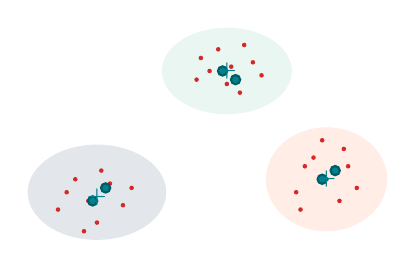
\begin{tikzpicture}[
    enemy/.style={circle, fill=AlertRed, minimum size=3pt, inner sep=0pt},
    jammer/.style={circle, fill=CyberTeal, minimum size=6pt, inner sep=0pt, draw=CyberTeal!70!black, thick},
    scale=0.55, every node/.style={scale=0.55}
]
  % Cluster 1 (bottom-left)
  \fill[MARLBlue, opacity=0.12] (1.2,1.2) ellipse (1.6 and 1.1);
  \foreach \x/\y in {0.3/0.8, 0.7/1.5, 1.2/0.5, 1.5/1.4, 1.0/1.0, 0.5/1.2, 1.8/0.9, 1.3/1.7, 0.9/0.3, 2.0/1.3}{
    \node[enemy] at (\x,\y) {};
  }
  \node[jammer] at (1.1,1.0) {}; \node[jammer] at (1.4,1.3) {};

  % Cluster 2 (top-center)
  \fill[JammerGreen, opacity=0.12] (4.2,4.0) ellipse (1.5 and 1.0);
  \foreach \x/\y in {3.5/3.8, 4.0/4.5, 4.5/3.5, 4.8/4.2, 3.8/4.0, 4.2/3.7, 4.6/4.6, 3.6/4.3, 4.3/4.1, 5.0/3.9}{
    \node[enemy] at (\x,\y) {};
  }
  \node[jammer] at (4.1,4.0) {}; \node[jammer] at (4.4,3.8) {};

  % Cluster 3 (right)
  \fill[SignalOrange, opacity=0.12] (6.5,1.5) ellipse (1.4 and 1.2);
  \foreach \x/\y in {5.8/1.2, 6.2/2.0, 6.8/1.0, 7.0/1.8, 6.5/1.5, 6.0/1.8, 6.9/2.2, 7.2/1.3, 5.9/0.8, 6.4/2.4}{
    \node[enemy] at (\x,\y) {};
  }
  \node[jammer] at (6.4,1.5) {}; \node[jammer] at (6.7,1.7) {};

  % Centroid markers
  \node[font=\Large\bfseries, CyberTeal] at (1.2,1.1) {+};
  \node[font=\Large\bfseries, CyberTeal] at (4.2,4.0) {+};
  \node[font=\Large\bfseries, CyberTeal] at (6.5,1.5) {+};
\end{tikzpicture}
\end{center}

\vspace{0.1cm}
\footnotesize
$\varepsilon = 30\,$m (neighborhood radius)\\
$\mathrm{minPts} = 2$ (minimum cluster size)\\
$k = 3$ clusters detected\\
$M = 6$ jammers $\to$ 2 per cluster

\column{0.55\textwidth}
\begin{block}{\small Why DBSCAN?}
  \footnotesize
  \begin{itemize}
    \item Enemy swarms naturally form \alert{spatial clusters}.
    \item Random jammer placement wastes the first 100--200 steps just repositioning.
    \item DBSCAN finds cluster structure from enemy $(x,y)$ positions --- \textbf{no labels needed}.
    \item Jammers start at centroids $\to$ immediately in effective range.
  \end{itemize}
\end{block}

\vspace{0cm}
\begin{exampleblock}{\small DBSCAN Algorithm --- 3 Steps}
  \footnotesize
  \begin{enumerate}
    \item For each drone, find all drones within $\varepsilon = 30\,$m.
    \item If $\geq$ minPts$=2$ neighbors $\to$ core point $\to$ form cluster.
    \item Compute centroid $\mu_k$ of each cluster $k$.
  \end{enumerate}
  \vspace{0.05cm}
  Place jammers at $\mu_k \pm$ small random offset.\\
  Re-run every 10 timesteps as swarm moves.
\end{exampleblock}
\end{columns}
\end{frame}

% ============================================================
\section{IV : Agent Design --- Observation, Actor \& Critic}\label{sec:agents}
% ============================================================

\begin{frame}{What Each Jammer Sees --- 5D State Observation}
\vspace{-0.1cm}
\begin{center}
\footnotesize
\renewcommand{\arraystretch}{1.35}
\setlength{\tabcolsep}{3pt}
\begin{tabular}{|c|l|l|c|p{4.8cm}|}
\hline
\rowcolor{MARLBlue!15}
\textbf{Index} & \textbf{Feature} & \textbf{Formula} & \textbf{Range} & \textbf{Meaning} \\
\hline
$s[0]$ & dist\_to\_centroid  & $\|\mathbf{p}_j - \mu_k\| \,/\, \text{arena}$ & $[0,1]$ & How far am I from my assigned cluster center? \\
\hline
$s[1]$ & cluster\_density    & $n_k \,/\, N$                                   & $[0,1]$ & What fraction of enemies are in my cluster? \\
\hline
$s[2]$ & dist\_to\_others    & $\overline{\|\mathbf{p}_j - \mathbf{p}_{j'}\|} \,/\, \text{arena}$ & $[0,1]$ & How spread out am I from teammate jammers? \\
\hline
$s[3]$ & coverage\_overlap   & pairs within $2 R_{\text{jam}}$ / total          & $[0,1]$ & Am I wasting coverage by overlapping a teammate? \\
\hline
$s[4]$ & band\_match         & $\mathbf{1}[b_j = b_{\text{enemy}}]$            & $\{0,1\}$ & Is my frequency matching the enemy band? \\
\hline
\end{tabular}
\end{center}

\vspace{0.3cm}
\begin{exampleblock}{Normalization}
  \centering\small
  All values clipped to $[0,\,1]$ before entering the neural network:\quad
  $\mathbf{s}_{\text{norm}} = \mathrm{clip}(\mathbf{s},\;0,\;1)$\\[3pt]
  Prevents any single feature from dominating the network activations.
\end{exampleblock}
\end{frame}

% ──────────────────────────────────────────────────────────────
\begin{frame}{Actor Network --- Mapping 5D Observation to Actions}
\begin{columns}[T,onlytextwidth]
\column{0.58\textwidth}
\vspace{0.1cm}
\begin{center}
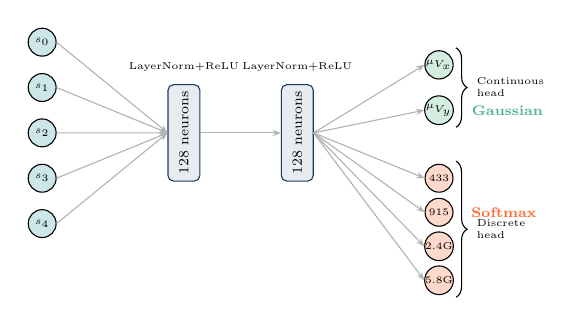
\begin{tikzpicture}[
    neuron/.style={circle, draw, minimum size=14pt, inner sep=0pt, font=\tiny},
    hidden/.style={rectangle, rounded corners=2pt, draw=MARLBlue, fill=MARLBlue!10,
                   minimum width=16pt, minimum height=42pt, font=\scriptsize},
    output/.style={circle, draw, minimum size=14pt, inner sep=0pt, font=\tiny},
    conn/.style={-{Stealth[length=3pt]}, thin, gray!60},
    label/.style={font=\scriptsize, align=center},
    scale=0.72, every node/.style={scale=0.72}
]
  % Input neurons
  \foreach \i/\lab in {1/s_0, 2/s_1, 3/s_2, 4/s_3, 5/s_4}{
    \node[neuron, fill=CyberTeal!20] (i\i) at (0, -\i*0.8+0.4) {$\lab$};
  }
  % Hidden layers
  \node[hidden] (h1) at (2.5,-2) {\rotatebox{90}{128 neurons}};
  \node[label, above=2pt] at (h1.north) {\tiny LayerNorm+ReLU};
  \node[hidden] (h2) at (4.5,-2) {\rotatebox{90}{128 neurons}};
  \node[label, above=2pt] at (h2.north) {\tiny LayerNorm+ReLU};

  % Output neurons — continuous
  \node[output, fill=JammerGreen!25] (ov1) at (7,-0.8) {$\mu_{V_x}$};
  \node[output, fill=JammerGreen!25] (ov2) at (7,-1.6) {$\mu_{V_y}$};
  % Output neurons — discrete
  \node[output, fill=SignalOrange!25] (ob1) at (7,-2.8) {\tiny 433};
  \node[output, fill=SignalOrange!25] (ob2) at (7,-3.4) {\tiny 915};
  \node[output, fill=SignalOrange!25] (ob3) at (7,-4.0) {\tiny 2.4G};
  \node[output, fill=SignalOrange!25] (ob4) at (7,-4.6) {\tiny 5.8G};

  % Connections
  \foreach \i in {1,...,5}{
    \draw[conn] (i\i.east) -- (h1.west);
  }
  \draw[conn] (h1.east) -- (h2.west);
  \draw[conn] (h2.east) -- (ov1.west);
  \draw[conn] (h2.east) -- (ov2.west);
  \draw[conn] (h2.east) -- (ob1.west);
  \draw[conn] (h2.east) -- (ob2.west);
  \draw[conn] (h2.east) -- (ob3.west);
  \draw[conn] (h2.east) -- (ob4.west);

  % Labels
  \node[label, right=4pt] at (ov2.east) {\textcolor{JammerGreen}{\textbf{Gaussian}}};
  \node[label, right=4pt] at (ob2.east) {\textcolor{SignalOrange}{\textbf{Softmax}}};

  % Bracket labels
  \draw[decorate, decoration={brace, amplitude=4pt}] (7.3,-0.5) -- (7.3,-1.9)
    node[midway, right=5pt, font=\tiny, align=left]{Continuous\\head};
  \draw[decorate, decoration={brace, amplitude=4pt}] (7.3,-2.5) -- (7.3,-4.9)
    node[midway, right=5pt, font=\tiny, align=left]{Discrete\\head};
\end{tikzpicture}
\end{center}

\column{0.40\textwidth}
\begin{block}{Layer Sizes}
  \footnotesize
  $5 \to 128$: each neuron learns a specific combination of the 5 input features.\\[3pt]
  $128 \to 128$: second layer combines simple patterns into complex jamming strategies.\\[3pt]
  \textbf{Total:} $(5 \times 128) + (128 \times 128) + (128 \times 6)$\\
  $\approx$ \alert{18{,}000} trainable weights.
\end{block}
\end{columns}

\vspace{0.2cm}
\begin{center}
\fcolorbox{GoldHighlight}{LightGray}{%
  \parbox{0.9\textwidth}{%
    \centering\footnotesize
    \textbf{Parameter sharing:} all $M=6$ jammers use \alert{ONE} Actor network.
    Each jammer passes its own local 5D observation.
    Different inputs $\to$ different actions $\to$ coordinated behaviour.
  }%
}
\end{center}
\end{frame}

% ──────────────────────────────────────────────────────────────
\begin{frame}{Critic Network --- Estimating Team Value $V(s)$}
\begin{columns}[T,onlytextwidth]
\column{0.55\textwidth}

\begin{center}
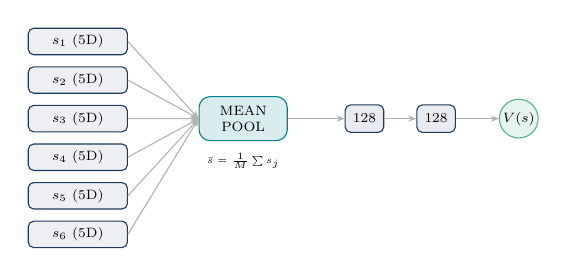
\begin{tikzpicture}[
    state/.style={rectangle, rounded corners=2pt, draw=MARLBlue, fill=MARLBlue!8,
                  minimum width=1.8cm, minimum height=0.4cm, font=\scriptsize, align=center},
    pool/.style={rectangle, rounded corners=4pt, draw=CyberTeal, fill=CyberTeal!15,
                 minimum width=1.6cm, minimum height=0.8cm, font=\scriptsize, align=center},
    hidden/.style={rectangle, rounded corners=2pt, draw=MARLBlue, fill=MARLBlue!10,
                   minimum width=0.7cm, minimum height=0.5cm, font=\scriptsize},
    val/.style={circle, draw=JammerGreen, fill=JammerGreen!15, minimum size=20pt,
                font=\scriptsize, inner sep=0pt},
    conn/.style={-{Stealth[length=3pt]}, thin, gray!60},
    scale=0.70, every node/.style={scale=0.70}
]
  % Jammer states
  \foreach \i in {1,...,6}{
    \node[state] (s\i) at (0, -\i*0.7+0.35) {$s_\i$ (5D)};
  }
  % Mean pool
  \node[pool] (mp) at (3,-1.75) {MEAN\\POOL};
  \node[font=\tiny, below=2pt] at (mp.south) {$\bar{s} = \frac{1}{M}\sum s_j$};
  % Hidden
  \node[hidden] (h1) at (5.2,-1.75) {128};
  \node[hidden] (h2) at (6.5,-1.75) {128};
  % V(s)
  \node[val] (v) at (8,-1.75) {$V(s)$};

  \foreach \i in {1,...,6}{
    \draw[conn] (s\i.east) -- (mp.west);
  }
  \draw[conn] (mp.east) -- (h1.west);
  \draw[conn] (h1.east) -- (h2.west);
  \draw[conn] (h2.east) -- (v.west);
\end{tikzpicture}
\end{center}

\begin{exampleblock}{Why Mean Pooling?}
  \footnotesize
  Critic must see the whole team, but input size must stay fixed.
  Mean pool collapses $M \times 5 \to 5$ --- scales to \alert{any number of jammers} without retraining.
\end{exampleblock}

\column{0.43\textwidth}
\begin{block}{What Does $V(s)$ Mean?}
  \footnotesize
  $V(s) = 0.74$ means:\\
  \textit{"From this team configuration, I expect 0.74 total reward over the remaining episode."}\\[6pt]
  High $V(s)$ $\to$ jammers well positioned, correct bands, $\lambda_2$ already falling.\\[3pt]
  Low $V(s)$ $\to$ jammers misplaced, wrong frequency, $\lambda_2$ still high.
\end{block}
\end{columns}

\begin{center}
\fcolorbox{GoldHighlight}{LightGray}{%
  \parbox{0.92\textwidth}{%
    \centering\footnotesize
    \textbf{Centralized Training / Decentralized Execution (CTDE)}\\[3pt]
    \textbf{Training:} Critic uses pooled global state $\to$ better gradient estimates for Actor.

    \\
    \textbf{Deployment:} Critic is \alert{completely discarded} $\to$ each jammer runs Actor alone using only its own 5D observation.
  }%
}
\end{center}
\end{frame}

% ============================================================
\section{V : Reward Function \& TD Learning}\label{sec:training}
% ============================================================

\begin{frame}{Reward Function --- 5 Terms Teaching the Agent What ``Good'' Means}
\vspace{-0.1cm}
\begin{center}
\footnotesize
\renewcommand{\arraystretch}{1.3}
\setlength{\tabcolsep}{3pt}
\begin{tabular}{|l|l|c|c|p{3.8cm}|}
\hline
\rowcolor{MARLBlue!15}
\textbf{Term} & \textbf{Formula} & \textbf{Weight} & \textbf{Dir.} & \textbf{Purpose} \\
\hline
$\lambda_2$ Reduction & $1 - \lambda_2(t)\,/\,\lambda_2(0)$ & $\omega_1 = 1.0$ & $\uparrow$ & \textbf{PRIMARY} --- swarm fragmentation \\
\hline
Band Match & $\frac{1}{M}\sum \mathbf{1}[b_j = b_{\text{enemy}}]$ & $\omega_2 = 0.3$ & $\uparrow$ & Correct frequency selection \\
\hline
Cluster Proximity & $\frac{1}{M}\sum \exp\!\left(-\kappa \cdot d_{\text{centroid}}\right)$ & $\omega_3 = 0.2$ & $\uparrow$ & Stay near assigned cluster \\
\hline
Energy Penalty & $\frac{1}{M}\sum \|\mathbf{v}_j\|^2 / v_{\max}^2$ & $\omega_4 = 0.1$ & $\downarrow$ & Discourage unnecessary movement \\
\hline
Overlap Penalty & overlapping pairs / total pairs & $\omega_5 = 0.2$ & $\downarrow$ & Spread coverage across clusters \\
\hline
\end{tabular}
\end{center}

\vspace{0.3cm}
\begin{block}{Total Reward}
  \centering
  $R(t) = \omega_1 \cdot (\lambda_2\text{ reduction}) + \omega_2 \cdot (\text{band match}) + \omega_3 \cdot (\text{proximity}) - \omega_4 \cdot (\text{energy}) - \omega_5 \cdot (\text{overlap})$
\end{block}
\end{frame}

% ──────────────────────────────────────────────────────────────
\begin{frame}{Temporal Difference Error --- How the Agent Measures Surprise}

\begin{exampleblock}{Core Idea}
  \centering\small
  The Critic predicts expected future reward at state $s_t$.
  After one step, we see what \alert{actually happened}.
  TD error = gap between prediction and reality.
\end{exampleblock}

\vspace{0.15cm}
\begin{columns}[T,onlytextwidth]
\column{0.55\textwidth}
\footnotesize
\textbf{Step 1 --- Critic prediction at time $t$:}\\
$V(s_t)$ = ``From this state, I expect $X$ total future reward''\\[6pt]
\textbf{Step 2 --- Better estimate after one step:}
\[
  G_t \approx r_t + \gamma \cdot V(s_{t+1})
\]
$r_t$ = actual reward; $\gamma = 0.99$\\[6pt]
\textbf{Step 3 --- TD Error:}
\[
  \boxed{\delta_t = r_t + \gamma \cdot V(s_{t+1}) - V(s_t)}
\]

\column{0.43\textwidth}
\begin{exampleblock}{\centering $\delta_t > 0$ --- {Better than expected}}
  \footnotesize Action was good $\to$ increase its probability.
\end{exampleblock}

\vspace{0.1cm}
\begin{block}{\centering $\delta_t = 0$ --- Matched prediction}
  \footnotesize Action was average $\to$ no change needed.
\end{block}

\vspace{0.1cm}
\begin{alertblock}{\centering $\delta_t < 0$ --- {Worse than expected}}
  \footnotesize Action was bad $\to$ decrease its probability.
\end{alertblock}
\end{columns}

\vspace{0.2cm}
\begin{center}
\fcolorbox{GoldHighlight}{LightGray}{%
  \parbox{0.92\textwidth}{%
    \centering\footnotesize
    $\delta_t$ is computed for \textbf{every timestep} in the buffer after each rollout.
    It is the raw signal from which Advantage and GAE are both derived.
    \alert{Without $\delta_t$ there is no learning signal} --- it is the engine of all RL.
  }%
}
\end{center}
\end{frame}

% ──────────────────────────────────────────────────────────────
\begin{frame}{From TD Error to GAE --- Computing How Good Each Action Truly Was}
\vspace{-0.2cm}
\begin{columns}[T,onlytextwidth]
\column{0.48\textwidth}
\begin{alertblock}{\footnotesize Why Not Use $\delta_t$ Directly?}
  \scriptsize
  $\delta_t$ is only \alert{one step} of information.\\
  It fully trusts $V(s_{t+1})$, which is estimated by the Critic.\\[3pt]
  Early in training $\to$ Critic is wrong $\to$ $\delta_t$ is wrong $\to$ bad learning signal.\\[3pt]
  We need to \textbf{look further ahead} for a more accurate signal.
\end{alertblock}

\vspace{-0.1cm}
\begin{block}{\footnotesize Advantage $A_t$}
  \scriptsize
  $A_t$ = ``How much \alert{better} was THIS action compared to average?''\\[3pt]
  $A_t > 0$ $\to$ above average $\to$ reinforce\\
  $A_t < 0$ $\to$ below average $\to$ suppress\\[3pt]
  True: $A_t = Q(s_t, a_t) - V(s_t)$\\
  But $Q$ is unknown $\to$ we must \textbf{estimate} it.
\end{block}

\column{0.50\textwidth}
\begin{exampleblock}{\footnotesize Generalised Advantage Estimation (GAE)}
  \scriptsize
  1-step: $\hat{A}_t^{(1)} = \delta_t$\\[2pt]
  2-step: $\hat{A}_t^{(2)} = \delta_t + \gamma\delta_{t+1}$\\[2pt]
  $n$-step: $\hat{A}_t^{(n)} = \sum_{l=0}^{n-1} \gamma^l \delta_{t+l}$\\[6pt]
  \textbf{GAE} --- exponentially weighted sum of all $n$-step estimates:
  \[
    \boxed{A_t^{\text{GAE}} = \delta_t + (\gamma\lambda)\,A_{t+1}^{\text{GAE}}}
  \]
  Computed \alert{backwards} from $t=T$ to $t=0$.
\end{exampleblock}
\end{columns}

\vspace{0cm}
\begin{center}
\fcolorbox{GoldHighlight}{LightGray}{%
  \parbox{0.94\textwidth}{%
    \centering\scriptsize
    \textbf{Example --- last 4 steps:}\quad
    $\delta_{47}\!=\!-0.02$,\; $\delta_{48}\!=\!+0.15$,\; $\delta_{49}\!=\!+0.41$,\; $\delta_{50}\!=\!0$\\[2pt]
    $A_{50}=0$\quad
    $A_{49}=0.41$\quad
    $A_{48}=0.15+0.94\!\times\!0.41=\mathbf{+0.535}$\quad
    $A_{47}=-0.02+0.94\!\times\!0.535=\mathbf{+0.483}$\\[2pt]
    Step 47 looks bad in isolation ($\delta\!=\!-0.02$), but GAE shows it was \alert{actually good} ($+0.483$) because it set up the big reward at step 49.
  }%
}
\end{center}
\end{frame}

% ============================================================
\section{VI : PPO --- Proximal Policy Optimization}\label{sec:ppo}
% ============================================================
% Slide 13a
% ============================================================

\begin{frame}[t]{PPO --- Why Standard Policy Gradient Breaks}

\normalsize

\begin{alertblock}{Standard Policy Gradient}
\[
\theta \leftarrow \theta + \alpha A_t \nabla_\theta \log \pi_\theta(a_t|s_t)
\]

Large $A_t$ $\Rightarrow$ very large update $\Rightarrow$ policy changes drastically.

\textbf{Issue:} No control over how much policy changes per update.
\end{alertblock}

\vspace{0cm}

\begin{columns}[T,onlytextwidth]

% ---- LEFT SIDE ----
\column{0.50\textwidth}

\begin{exampleblock}{PPO Fix --- Probability Ratio}

\vspace{0.1cm}

\[
r_t(\theta)=
\frac{\pi_\theta(a_t|s_t)}
{\pi_{\theta_{\text{old}}}(a_t|s_t)}
\]

\vspace{0.2cm}

\centering
\large
\alert{$r_t \in [0.8,1.2]$ ensures policy changes $\le 20\%$ per update}

\end{exampleblock}

% ---- RIGHT SIDE ----
\column{0.48\textwidth}

\begin{block}{Four Cases}

\small
\renewcommand{\arraystretch}{1.4}

\begin{tabular}{llll}
\hline
$A_t$ & $r_t$ & PPO Behaviour & Result\\
\hline
$+$ large & 1.8 & clipped to 1.2 & capped\\
$+$ small & 1.1 & not clipped & allowed\\
$-$ large & 0.3 & clipped to 0.8 & capped\\
$-$ small & 0.9 & not clipped & allowed\\
\hline
\end{tabular}

\end{block}

\end{columns}

\end{frame}
% ============================================================
% Slide 13b
% ============================================================

\begin{frame}[t]{PPO --- Clipped Objective}

\footnotesize

\begin{block}{Clipped Objective}

\[
L^{CLIP} =
\mathbb{E}_t
\Big[
\min(
r_t(\theta)A_t,
clip(r_t,0.8,1.2)A_t
)
\Big]
\]

\smallskip

min() picks the \alert{more conservative} term.

\smallskip

$\epsilon=0.2$ $\Rightarrow$ trust region $[0.8,1.2]$  
$\Rightarrow$ stable policy improvement.

\end{block}

\vspace{0.15cm}

\begin{exampleblock}{Entropy Bonus}

\[
H(\pi)=-\sum_a \pi(a|s)\log\pi(a|s)
\]

\vspace{0.15cm}

\begin{itemize}
\item High entropy $\Rightarrow$ exploration
\item Low entropy $\Rightarrow$ policy collapse
\end{itemize}

\vspace{0.1cm}

\[
L_{entropy}=-c_1H(\pi), \quad c_1=0.01
\]

\end{exampleblock}

\end{frame}


% ============================================================
% Slide 13c
% ============================================================

\begin{frame}[t]{PPO --- Critic Loss and Complete Objective}

\footnotesize
\vspace{-0.3cm}
\begin{columns}[T,onlytextwidth]

% ---- LEFT COLUMN ----
\column{0.45\textwidth}

\begin{block}{Critic Loss --- Value Estimation}

\[
L_{\text{critic}} =
\frac{1}{T}\sum_t (V(s_t) - G_t)^2
\]

\smallskip

$G_t = A_t + V(s_t)$  (target return)

\smallskip

\textbf{Interpretation}

\begin{itemize}
\item $V(s_t)$ → predicted value
\item $G_t$ → actual return
\item Critic learns to minimize prediction error
\end{itemize}

Weight: $c_2 = 0.5$ (critic supports actor)

\end{block}

% ---- RIGHT COLUMN ----
\column{0.51\textwidth}

\begin{block}{Optimization Tricks}

\textbf{1. Negative sign on $L^{CLIP}$}

PyTorch minimizes loss, but PPO must maximize policy objective.
\vspace{0cm}
\[
\text{Optimize } -L^{CLIP}
\]

\smallskip

\textbf{2. Gradient Clipping}

If gradient norm becomes too large:
\vspace{-0.2cm}
\[
||\nabla|| > 0.5
\]

scale gradients to keep updates stable.

\end{block}

\end{columns}

\vspace{-0.1cm}

% ---- FINAL PPO LOSS ----

\begin{center}

\fcolorbox{black}{gray!10}{
\parbox{0.95\linewidth}{
\centering
\normalsize
\textbf{Complete PPO Loss}
\vspace{-0.2cm}
\[
L_{\text{total}}
=
-L^{CLIP}
+
0.5L_{\text{critic}}
-
0.01L_{\text{entropy}}
\]

\footnotesize
\quad • \quad Actor improves policy \quad • \quad
Critic improves value estimates \quad • \quad
Entropy maintains exploration
}}

\end{center}

\end{frame}
% ============================================================
\section{VII : Training Results \& Evaluation}\label{sec:results}
% ============================================================

% --- Slide 1 ---
\begin{frame}{Training Results: $\lambda_2$ vs Training Episodes}
\begin{figure}
  \centering
  
\includegraphics[width=0.75\linewidth]{01_lambda2_vs_episodes.png}
  \caption{\scriptsize $\lambda_2$ vs.\ Training Episodes}
\end{figure}
\end{frame}

% --- Slide 2 ---
\begin{frame}{Training Results: Reward vs Training Episodes}
\begin{figure}
  \centering
  
\includegraphics[width=0.75\linewidth]{02_reward_vs_episodes.png}
  \caption{\scriptsize Reward vs.\ Training Episodes}
\end{figure}
\end{frame}

% --- Slide 3 ---
\begin{frame}{Training Results: Average Power Comparison}
\begin{figure}
  \centering
  
\includegraphics[width=0.75\linewidth]{04_avg_power_comparison.png}
  \caption{\scriptsize Average Power Comparison}
\end{figure}
\end{frame}

% --- Slide 4 ---
\begin{frame}{Training Results: Connectivity Before vs After}
\begin{figure}
  \centering
  
\includegraphics[width=0.95\linewidth]{05_connectivity_before_after.png}
  \caption{\scriptsize Connectivity Before vs.\ After}
\end{figure}
\end{frame}

% ──────────────────────────────────────────────────────────────
\begin{frame}{Dataset Evaluation (Military Drone Swarm \& Saturation Attack Dataset)}
\begin{columns}[T,onlytextwidth]
\column{0.48\textwidth}
\begin{figure}
  \centering
  
\includegraphics[width=1.05\linewidth]{01_lambda2_vs_scenarios.png}
  \vspace{-0.3cm}
  \caption{\scriptsize $\lambda_2$ vs.\ Training Episodes}
\end{figure}

\column{0.48\textwidth}
\begin{figure}
  \centering
  
\includegraphics[width=1.05\linewidth]{02_reward_vs_scenarios.png}
  \vspace{-0.3cm}
  \caption{\scriptsize Reward vs.\ Training Episodes}
\end{figure}
\end{columns}


\end{frame}

% ============================================================
% THANK YOU
% ============================================================
{\setbeamercolor{palette primary}{fg=white, bg=DeepNavy}
\begin{frame}[standout]
  \Huge Thank You\\[0.6cm]
  \large Questions \& Discussion
\end{frame}
}

\end{document}
